\documentclass{article}
\usepackage[T1]{fontenc}
\usepackage{times}
\usepackage{geometry}
\geometry{a4paper,left=0.6cm,right=0.7cm,top=1.5cm,bottom=1cm,columnsep=0.8cm}
\usepackage[utf8]{inputenc}
\usepackage{textcomp}
\usepackage{newtxtext}
\usepackage{fontawesome}          % icônes de base seulement
\usepackage[hidelinks]{hyperref}
\usepackage{multicol}
\usepackage{tikz}
\usepackage{hyphsubst}
\usepackage{moresize}
\usepackage{hyphenat}
\usepackage{tabularx}
\usepackage{ragged2e}
\usepackage{xcolor}
\usepackage{enumitem}
\usetikzlibrary{calc, positioning}
\newcolumntype{Y}{>{\RaggedRight\arraybackslash}X}

% icônes manquantes -> puce
\makeatletter
\@for\sym:=faBrain,faMicrochip,faHandshakeO,faTools,faNetworkWired,%
             faDatabase,faServer,faGit,faUsers,faComments,faCalendar,faGroup\do{%
  \@ifundefined{\sym}{\expandafter\newcommand\csname\sym\endcsname{\textbullet}}{}}
\makeatother

% couleurs
\definecolor{maincolor}{HTML}{f0fafc}
\definecolor{seccolor}{HTML}{ffffff}
\definecolor{gray}{HTML}{8c94a9}
\definecolor{sidetext}{HTML}{59cee5}

% bande latérale bleue
\usepackage{eso-pic}
\AddToShipoutPictureBG{%
  \begin{tikzpicture}[remember picture,overlay]
    \fill[maincolor] (current page.north west) rectangle
                     ([xshift=0.3\paperwidth] current page.south west);
  \end{tikzpicture}%
}

% listes
\setlist[itemize]{itemsep=-2pt,topsep=0pt,leftmargin=1.08cm}
\renewcommand{\labelitemi}{\textcolor{sidetext}{\footnotesize$\bullet$}}

\setlength{\parindent}{0pt}
\usepackage{paracol}
\columnratio{0.3}

\begin{document}
\pagestyle{empty}

\begin{paracol}{2}
% ────────────────────────────────────────
% Colonne gauche
% ────────────────────────────────────────
\color{sidetext}
\vspace*{-0.5cm}


\noindent
\begin{minipage}{\linewidth}
  \centering
  \ifx\relax1d45146ef137465999ebad5d6124254f.png\relax\else
  \begin{tikzpicture}
    \clip (0,0) circle (1.5cm) node[anchor=center]
      {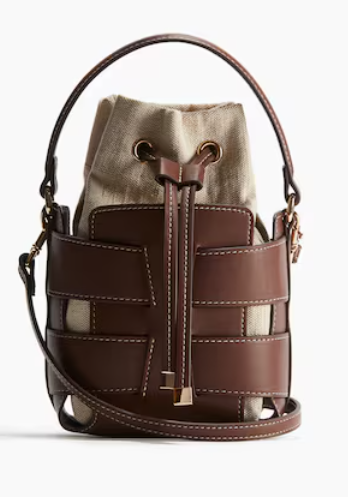
\includegraphics[width=3cm]{1d45146ef137465999ebad5d6124254f.png}};
  \end{tikzpicture}
  \fi

  \vspace{3mm}
  {\color{black}\LARGE \textbf{Judikael Mourouvin}}

  \vspace{1mm}
  {\large Technicien informatique spécialisé en marketing digital}

  \vspace{3mm}
  {\color{gray}\rule{\linewidth}{0.4pt}} \\
\end{minipage}

% ── Coordonnées
\begin{tabular}{@{}c l}
  \faPhone &
  \begin{tabular}[t]{@{}l@{}}
    {\color{gray}Téléphone} \\ +590 0690 91 14 48
  \end{tabular} \\
  \\
  \faLinkedin &
  \begin{tabular}[t]{@{}l@{}}
    {\color{gray}LinkedIn} \\
    \href{}{}
  \end{tabular} \\
  \\
  \faMapMarker &
  \begin{tabular}[t]{@{}l@{}}
    {\color{gray}Adresse} \\ Route de Cocoyer \\ 97190 Gosier
  \end{tabular} \\
  \\
  \faEnvelope &
  \begin{tabular}[t]{@{}l@{}}
    {\color{gray}Email} \\
    \href{mailto:jkmou971@gmail.com}{jkmou971@gmail.com}
  \end{tabular} \\
\end{tabular}

\vspace{2mm}
{\color{gray}\rule{\linewidth}{0.4pt}} \\

% ── Langues --------------------------------------------------------
{\color{black}{Langues}}

\vspace{2mm}
\begin{itemize}[leftmargin=*]
\item English - \textcolor{gray}{}
\item Espagnol - \textcolor{gray}{}\end{itemize}          % ← le placeholder va contenir \begin{itemize}…\end{itemize}
\vspace{2mm}
{\color{gray}\rule{\linewidth}{0.4pt}} \\

% ── Compétences ----------------------------------------------------
\vspace{2mm}
{\color{black}{Compétences Clés}}

\vspace{2mm}
\begin{itemize}[leftmargin=*]
\item Administration
\item Réseaux
\item Support
\item Maintenance
\item Diagnostic
\item Marketing
\item Configuration\end{itemize}              % ← idem, une vraie liste
\vspace{2mm}
{\color{gray}\rule{\linewidth}{0.4pt}} \\

% ── Centres d'intérêt
\vspace{2mm}
{\color{black}{Centres d’intérêt}}

\vspace{2mm}
\begin{itemize}[leftmargin=*]
\item Lecture
\item Sport
\item Musique
\item Voyage
\end{itemize}     % ← simple itemize ou tabular

\vfill
~

% ────────────────────────────────────────
\switchcolumn
% Colonne droite
% ────────────────────────────────────────
\color{black}

% ── Profil
\textcolor{black}{\Large \textbf{Profil Professionnel}} \\[2pt]
Passionné par l’informatique et le marketing digital, je possède une double compétence en administration des systèmes d’information et en communication numérique. Au sein de collectivités, d’organismes publics et de PME, j’ai piloté des projets digitaux, assuré le support utilisateur et maintenu des infrastructures. Autonome et rigoureux, je sais analyser les besoins, déployer les postes et optimiser les réseaux. Je souhaite désormais mettre mon savoir-faire au service de nouveaux défis à temps plein. \\[8pt]

% ── Expérience
\textcolor{black}{\Large \textbf{Expérience Professionnelle}} \\[2pt]
\colorbox{maincolor}{%
  \begin{minipage}{\linewidth}
    \noindent
    \textbf{Alternant en marketing digital}\hfill 09/2023 - 08/2024\\
    Mairie du Gosier – DSI\\[-0.3em]
    \begin{itemize}[leftmargin=*]
      \item Analysé les besoins des services et proposé des solutions numériques, renforçant la communication interne \item Assuré le support et formé les utilisateurs, réduisant les incidents récurrents \item Participé à la stratégie digitale, augmentant la visibilité des actions municipales
    \end{itemize}
  \end{minipage}}

\vspace{3mm}

\colorbox{maincolor}{%
  \begin{minipage}{\linewidth}
    \noindent
    \textbf{Animateur de la zone informatique}\hfill 09/2022 - 08/2023\\
    Pôle Emploi, Gosier\\[-0.3em]
    \begin{itemize}[leftmargin=*]
      \item Guidé les demandeurs d’emploi dans l’usage des outils digitaux, améliorant leur autonomie \item Configuré et maintenu le parc informatique, garantissant sa disponibilité \item Résolu les incidents matériels et logiciels pour assurer la continuité du service
    \end{itemize}
  \end{minipage}}

\vspace{3mm}

\colorbox{maincolor}{%
  \begin{minipage}{\linewidth}
    \noindent
    \textbf{Stagiaire informaticien}\hfill 09/2020 - 08/2021\\
    NUMERIKA, Baie-Mahault\\[-0.3em]
    \begin{itemize}[leftmargin=*]
      \item Installé et entretenu les équipements informatiques clients, diminuant les temps d’arrêt \item Géré le support de niveau 1 et les tickets dans les délais contractuels \item Rédigé les procédures de configuration pour faciliter la maintenance
    \end{itemize}
  \end{minipage}}   % ← blocs \colorbox{maincolor}{\begin{minipage}…}

\vspace{8mm}

% ── Formation
\textcolor{black}{\Large \textbf{Formation}} \\[2pt]
\colorbox{maincolor}{%
  \begin{minipage}{\linewidth}
    \noindent
    \textbf{Bachelor Marketing Digital}\hfill 09/2023 - 08/2024\\
    CFA IUTS\\[-0.3em]
    \begin{itemize}[leftmargin=*]
      \item Stratégies de communication digitale, gestion de contenu \item Analyse de données marketing et optimisation de campagnes \item Gestion de projets web et SEO
    \end{itemize}
  \end{minipage}}

\vspace{3mm}

\colorbox{maincolor}{%
  \begin{minipage}{\linewidth}
    \noindent
    \textbf{BTS Systèmes Numériques option Informatique \& Réseaux}\hfill 09/2019 - 06/2021\\
    Lycée de Chevalier Saint-Georges, Abymes\\[-0.3em]
    \begin{itemize}[leftmargin=*]
      \item Administration réseaux et systèmes \item Maintenance matérielle et logicielle \item Scripts et gestion de bases de données
    \end{itemize}
  \end{minipage}}       % ← lignes tabular par diplôme

\end{paracol}
\end{document}

